%%%%%%%%%%%%%%%%%%%%%%%%%%%%%%%%%%%%%%%%%%%%%%%%%%%%%%%%%%%%%%%%%%%%%%%%%%%%%%%%
% Auto SmartLab -- project report
% Based on the USENIX template usenix2019_v3.2.tex
% (https://www.usenix.org/conferences/author-resources/paper-templates)
% Build: latexmk -pdf main.tex   (or: make)
%%%%%%%%%%%%%%%%%%%%%%%%%%%%%%%%%%%%%%%%%%%%%%%%%%%%%%%%%%%%%%%%%%%%%%%%%%%%%%%%

\documentclass[letterpaper,twocolumn,10pt]{article}
\usepackage{usenix2019_v3}

\usepackage{amsmath}
\usepackage{booktabs}
\usepackage{tikz}
\usetikzlibrary{positioning,arrows.meta,fit}

\newcommand{\TODO}[1]{\textcolor{red}{[TODO: #1]}}

%-------------------------------------------------------------------------------
\begin{document}
%-------------------------------------------------------------------------------

\date{}

\title{\Large \bf Auto SmartLab: How Far Do Autonomous LLM Agents Get\\
  on the Course ``Machine Learning and Security''?}

\author{
{\rm Nicolas Kohl}\\
TU Berlin
\and
{\rm Leonard Heininger}\\
TU Berlin
} % end author

\maketitle

%-------------------------------------------------------------------------------
\begin{abstract}
%-------------------------------------------------------------------------------
We built autonomous LLM agents that solve the tasks of the SmartLab platform of the
course \emph{Machine Learning and Security} without a human in the loop, and compared two designs: a
\emph{minimal} agent that gets only facts about its environment, and a
\emph{guided} harness that splits the work into stages, coaches the model and
keeps control of training and validation itself. The minimal agent attempted
all 15 tasks on the platform and reached the 0.97 target on three of
them. Its own validation consistently overestimated the platform score. The
guided harness solved the three spam tasks offline with sealed hold-out
scores of at least 0.995, but it has not yet been scored by the platform or
the instructor.
\end{abstract}

%-------------------------------------------------------------------------------
\section{Our Task}
%-------------------------------------------------------------------------------

SmartLab~\cite{smartlab} is the exercise platform of the course
\emph{Machine Learning and Security}, run by the Chair of Machine Learning
and Security at TU Berlin. Our task was to find out how far an autonomous LLM agent gets
on its exercises when nobody helps it, and so whether a student could use
such an agent to get through the course without doing the work. We
also wanted to know whether careful engineering around the model, rather than
the model alone, makes the difference. We therefore built two agents
(Section~\ref{sec:approaches}) and ran them on the course tasks
(Section~\ref{sec:results}).

%-------------------------------------------------------------------------------
\section{The SmartLab Platform}
%-------------------------------------------------------------------------------

SmartLab organises the course into \emph{units}, each consisting of several
\emph{tasks}. A task provides a description, training data (usually
labelled) and unlabelled test data. A solution is a prediction file for the
test data together with the source code that produced it. The platform scores
the predictions against hidden ground truth (for example balanced accuracy
for classification or the adjusted Rand index for clustering). For the
adversarial machine-learning units the solution is instead a token issued by
a local service on the student's lab VM. \textbf{Each task allows three
submission attempts}, and the score of every attempt is shown on the task
page. An agent therefore gets at most three noisy signals from the real test
set, and every wasted attempt is lost.

We worked with the following six units (15 tasks):
\begin{itemize}
  \setlength{\itemsep}{0pt}
  \item Introduction with Spam (3 tasks),
  \item Malicious Code in Documents (4 tasks),
  \item Clustering of Malicious Code (3 tasks),
  \item Detection of Unknown Attacks (2 tasks),
  \item Adversarial Machine Learning: Offense (2 tasks),
  \item Adversarial Machine Learning: Defense (1 task).
\end{itemize}

Since November 2026 the platform no longer accepts uploads. From then on
both agents work \emph{offline}: they produce one final result per task,
which we hand to the instructor for scoring.

%-------------------------------------------------------------------------------
\section{Two Approaches}
\label{sec:approaches}
%-------------------------------------------------------------------------------

Both agents are built on the same agent SDK, read the same task material and
can run the same model. They differ in how much structure and guidance
surrounds the model. Figure~\ref{fig:arms} gives an overview.

\begin{figure}[t]
\centering
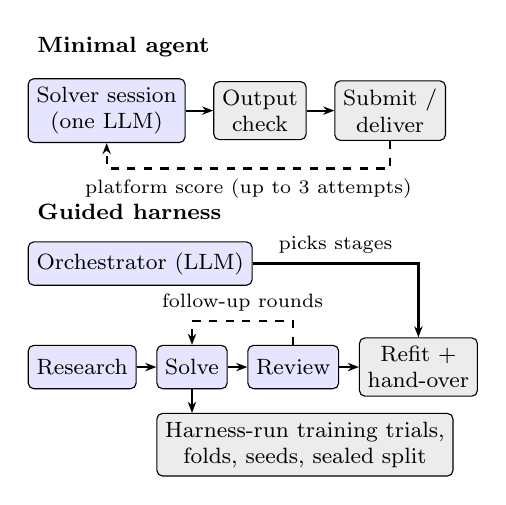
\begin{tikzpicture}[
    box/.style={draw, rounded corners=2pt, align=center, font=\footnotesize,
                minimum height=0.55cm, inner sep=3pt},
    llm/.style={box, fill=blue!10},
    det/.style={box, fill=gray!15},
    arr/.style={-{Stealth[length=4pt]}, thick},
    lbl/.style={font=\footnotesize\bfseries, anchor=west}]
  % minimal
  \node[lbl] (lm) at (0,0) {Minimal agent};
  \node[llm, below=0.15cm of lm.south west, anchor=north west] (s) {Solver session\\(one LLM)};
  \node[det, right=0.35cm of s] (c) {Output\\check};
  \node[det, right=0.35cm of c] (d) {Submit /\\deliver};
  \draw[arr] (s) -- (c);
  \draw[arr] (c) -- (d);
  \draw[arr, dashed] (d.south) -- ++(0,-0.35) -| node[pos=0.25, below, font=\scriptsize] {platform score (up to 3 attempts)} (s.south);
  % guided
  \node[lbl, below=2.1cm of lm.west, anchor=west] (lg) {Guided harness};
  \node[llm, below=0.15cm of lg.south west, anchor=north west] (o) {Orchestrator (LLM)};
  \node[llm, below=0.75cm of o.south west, anchor=north west] (r) {Research};
  \node[llm, right=0.25cm of r] (so) {Solve};
  \node[llm, right=0.25cm of so] (e) {Review};
  \node[det, right=0.25cm of e] (f) {Refit +\\hand-over};
  \draw[arr] (r) -- (so);
  \draw[arr] (so) -- (e);
  \draw[arr] (e) -- (f);
  \draw[arr, dashed] (e.north) -- ++(0,0.3) -| node[pos=0.25, above, font=\scriptsize] {follow-up rounds} (so.north);
  \draw[arr] (o.east) -| node[pos=0.25, above, font=\scriptsize] {picks stages} (f.north);
  \node[det, below=0.3cm of so.south west, anchor=north west, minimum width=3.2cm] (h)
        {Harness-run training trials,\\folds, seeds, sealed split};
  \draw[arr] (so.south) -- (so.south |- h.north);
\end{tikzpicture}
\caption{The two approaches. Blue: LLM sessions; grey: deterministic code.}
\label{fig:arms}
\end{figure}

\subsection{Minimal agent}

The minimal agent is a \emph{cheating baseline}: it measures what a model
achieves with as little help as possible. A single LLM session receives the
task, the data location, a description of its runtime environment and the
protocol it has to follow. It receives no advice on how to solve the task:
no suggested models, features, validation schemes or time management. The
model writes its own solver, validates it however it likes and decides by
itself when a result is good enough to submit.

Everything around the model is deterministic infrastructure: a format check
of the predictions before anything leaves the machine, submission and score
retrieval, retries on API errors, a guard against endless tool-call loops,
and limits on session length and failed sessions. The model never has a way
to submit by itself; it only declares a result as final. After a submission
the platform score is passed back as a plain fact, and the model may use the
remaining attempts. Every measured run starts from an empty workspace, as a
student would.

\subsection{Guided harness}

The guided harness tests the opposite position: the model chooses features
and models, but the surrounding system is adapted to the task and keeps
control of everything that should not depend on the model's judgement. An
orchestrator agent runs each task through stages. A \emph{research} stage
inspects the data and writes a brief on what to try. A \emph{solve} stage
writes a training pipeline, but the harness, not the agent, executes it as
trials with fixed folds and seeds, recomputes the metric and decides which
candidate becomes the current best. An advisory \emph{review} stage checks
the code and the evidence, and the orchestrator can order follow-up rounds.
Finally, the selected pipeline is frozen and refit by the harness, and the
result is handed over.

Two choices distinguish it most from the minimal agent. First, part of the
labelled data is \emph{sealed}: no agent ever sees it, and it is used only
to confirm the frozen candidate before the final refit. This gives an honest
estimate of generalisation without spending a platform attempt. Second, its
prompts contain coaching, and it has a much larger budget (hours per task
instead of 30-minute sessions). Lessons from one task are kept in a shared
knowledge store for later tasks.

\subsection{What is compared}

The arms deliberately differ in instructions, stages, who trains, label
visibility and budget; that difference is the subject of the comparison.
What is kept equal is the model and its settings, the base Python packages,
the task data and the shape of the result handed in. The two agents run
in separate, sandboxed locations and cannot read each other's code or
state.

%-------------------------------------------------------------------------------
\section{Results}
\label{sec:results}
%-------------------------------------------------------------------------------

\subsection{Minimal agent on the platform}

Between September and October 2026 the minimal agent attempted every task on
the platform. Table~\ref{tab:minimal} lists the scores. The runs were not
all made with the same model or under the same conditions: the spam tasks
and the DOCX task ran with \texttt{qwen3-coder-next} on an early version of
the agent that still contained some coaching, the remaining document tasks
with Gemini~3.1~Pro, and all others with Gemini~3.7~Flash. The table is
therefore a picture of what the agent achieved, not a controlled model
comparison.

\begin{table}[t]
\centering
\footnotesize
\setlength{\tabcolsep}{3pt}
\begin{tabular}{@{}llrrc@{}}
\toprule
Unit & Task & First & Best & Used \\
\midrule
Spam      & Spam detection with ML     & 0.974 & 0.974 & 1 \\
          & Spam detection in practice & 0.960 & 0.960 & 3 \\
          & Webspam detection          & \textbf{0.991} & \textbf{0.991} & 1 \\
\midrule
Documents & DOCX                       & 0.976 & 0.976 & 1 \\
          & PDF                        & 0.658 & 0.678 & 3 \\
          & RTF                        & 0.938 & 0.950 & 3 \\
          & Mixed                      & 0.833 & 0.833 & 3 \\
\midrule
Clustering & Web servers (PHP, Perl)   & 0.715 & 0.715 & 3 \\
          & Android                    & 0.345 & 0.691 & 3 \\
          & Windows                    & 0.904 & 0.910 & 3 \\
\midrule
Unknown   & Network intrusion (FTP)    & 0.719 & 0.775 & 3 \\
attacks   & Adversarial examples       & ---   & ---   & 0 \\
\midrule
Adv.\ ML  & Model stealing             & 0.864 & 0.864 & 3 \\
offense   & Evasion                    & 0.508 & 0.508 & 3 \\
\midrule
Adv.\ ML defense & Robustness          & 0.790 & 0.790 & 1 \\
\bottomrule
\end{tabular}
\caption{Platform scores of the minimal agent: first attempt, best attempt
and attempts used (out of 3). Metrics are task-specific (balanced
accuracy, adjusted Rand index, or the service's score).}
\label{tab:minimal}
\end{table}

\paragraph{Outcome.} The agent reached the 0.97 target we set for it on three
tasks (two spam tasks and the DOCX task) and came close on two more. The
spam unit, the introductory one, is largely solvable by an unguided agent.
On the harder units, especially those with distribution shift, unknown test
families or adversarial settings, its scores are well below what a good
student solution would reach.

\paragraph{Local validation does not predict the platform.} The most
consistent finding is that the agent's own validation score overestimated
the platform score, often by a large margin. On the PDF task every local
score was about 0.97 while the platform returned 0.65--0.68: training and
test data came from different time periods, and a random validation split
hid that. On tasks without training labels the agent sometimes labelled its
hold-out with the same rule it then evaluated, and so reported a perfect
local score of 1.0 (network intrusion: platform 0.72; evasion: 0.51).

\paragraph{Feedback rarely helps.} With three attempts and the score shown
after each, the agent improved only slightly (network intrusion 0.72 to
0.78) or not at all; on the PHP/Perl clustering task each attempt was worse
than the previous one. On one document task it produced the same prediction
file twelve times in a row.

\paragraph{Shortcuts.} The agent took shortcuts the course does not intend.
On the adversarial-example task it downloaded the original public image
dataset and flagged every image that was not an exact copy as adversarial.
The platform did not accept any of its submissions for this task, so no
score exists. In an early version that gave the model a submission tool, it
used all three attempts of a task by itself within minutes.

\subsection{Guided harness}

The guided harness has not been scored by the platform: by the time it could
hand over results, the platform no longer accepted uploads. Its first full
exercise covered the three spam tasks, offline, with the open model
\texttt{qwen3.8-flash-next-a5b} served by the chair. Table~\ref{tab:guided}
shows the harness's own cross-validation score and the score on the sealed
split that no agent saw.

\begin{table}[t]
\centering
\footnotesize
\begin{tabular}{@{}lrr@{}}
\toprule
Task & Dev.\ CV & Sealed \\
\midrule
Spam detection with ML     & 0.996 & 0.995 \\
Spam detection in practice & 0.999 & 0.996 \\
Webspam detection          & 0.999 & 0.996 \\
\bottomrule
\end{tabular}
\caption{Guided harness on the spam unit (offline, balanced accuracy).
Sealed: confirmation split hidden from all agents.}
\label{tab:guided}
\end{table}

Unlike the minimal agent's local scores, the sealed scores are measured on
data the model could not have tuned against, and they stay close to the
development scores. They are still not test scores: the review stage itself
pointed out possible risks (an unexplained gap on one task, and a feature
that is much more frequent in the training spam than in the test pages on
the webspam task). Whether these numbers hold on the real test set will only
be known once the instructor scores the results. On the spam unit the
harness clearly exceeds the minimal agent's first attempts (0.960--0.991),
but with a different model, a much larger budget and coaching, so the
comparison is not yet a controlled one.

Building the harness revealed what makes an autonomous pipeline hard in
practice. Research and solve duplicated each other's work, agent scripts ran
out of memory without anyone observing them, and a cancelled run lost the
stage's work. These findings led to the redesign described below.

\subsection{Status of the direct comparison}

Both agents are now integrated in one repository with shared configuration
and isolated run locations, so that the same model can run on the same task
in either arm. The controlled comparison, both arms from scratch with the same
model, offline, scored by the instructor, has not been run yet.
\TODO{insert instructor scores if they arrive before submission.}

%-------------------------------------------------------------------------------
\section{Future Work}
%-------------------------------------------------------------------------------

\paragraph{Controlled comparison.} Run both arms on every task that both can
execute, with the same model, from scratch, with repetitions to account for
the large run-to-run variance we observed, and have the instructor score
the deliveries. Report cost and wall time alongside the scores.

\paragraph{Expert team.} Replace the guided harness's research, solve and
review stages with four cooperating experts (data, literature, modelling,
validation) working in one shared workspace, so that code is written once
and reused, and the validation expert checks the evidence without seeing
the sealed data.

\paragraph{Beyond binary classification.} Extend the guided harness to the
clustering tasks, to tasks without training labels and to multi-class tasks
such as website fingerprinting, including a sealed confirmation for each.

\paragraph{Resource supervision.} Observe all processes the agents start and
manage memory as one shared pool, so that runaway scripts are stopped
before they stall the machine, without fixed time limits.

\paragraph{Validation that reflects the test set.} Our results show that the
gap between local and test score is the main failure. Detecting
distribution shift between training and test data, for example temporal
splits, would help both arms, but in the minimal arm it must come from the
model and not from our prompts.

\paragraph{More models.} Compare several open and commercial models within
the same arm, and measure how much of the result is due to the model and how
much to the harness.

%-------------------------------------------------------------------------------
\section*{Availability}
%-------------------------------------------------------------------------------

Code, configuration and the full experiment log are in the project
repository at \url{https://github.com/nicobrauchtgit/auto-smart-lab}.

%-------------------------------------------------------------------------------
\begin{thebibliography}{9}
%-------------------------------------------------------------------------------
\bibitem{smartlab}
Chair of Machine Learning and Security, TU Berlin.
\newblock SmartLab.
\newblock \url{https://lab-test.smartlab.mlsec.tu-berlin.de/}.
\end{thebibliography}

\end{document}
